\chapter{Non-linear modelling}
\label{chp:5}

\section{Introduction}
This chapter consists of  non-linear (beyond elasticity) modelling for the Finite Element Analysis with Abaqus including VUMAT. Additionally other analytical models are proposed to make a prediction for the non-linear behaviour of FFF products. 

\section{Methods and procedures}
\subsection{Finite Element Method}
The Finite Element Analysis was conducted in Abaqus in combination with a pre-written VUMAT according to the papers proposed by Melro \cite{Melro2012InfluenceMaterials}\cite{Melro2013}\cite{Melro2013MicromechanicalModelling}. 
%explicit and implicit
Explicit simulation including plasticity with yield and failure was implemented in a similar way to Melro's code. The main difference between explicit and implicit analysis is the dependency on time and increments. For static cases without plasticity the implicit method is often used, for dynamic cases including plasticity explicit method is used to determine the state of the material at every increment. Implicit simulations adopt a method called Euler integration scheme which ensures stability (unconditionally stable) and facilitates larger time steps. This method may be time consuming for dynamic loads.  Explicit analyses aims to solve for acceleration. Using simplifications, the acceleration of a body can be found for every increment, and additionally the velocity and displacement. This method is not unconditionally stable, and thus smaller time increments are required. This must be smaller than the Courant time step, which dictates the time taken by a sound wave to travel across an element. Explicit analysis offers a faster solution in events where there is a dynamic equilibrium. Since implicit has more trouble with non-linear material behaviour (as is plasticity) an explicit method was used \cite{Harish2019ImplicitMethod}. The Stable time increment of quasi-static analysis can be articifically increased by scaling the mass of the elements, allowing the stress wave to "travel" faster. The downside of this is the increase of kinetic energy introduced in the system, which should be below 10\% of the total energy.  
%Explanation of the VUMAT code

A VUMAT subroutine code was used in combination with ABAQUS to adjust constitutive models. A VUMAT is used if the abaqus material model library does not represent the behaviour of the material well, or if a user wants a more accurate response in a complex situation\cite{SimuliaWritingAbaqus}. Considering the very limited commercial models available for polymers, an adjusted VUMAT was implemented to simulate this behaviour. The VUMAT is written in academic coding language FORTRAN and makes use of inputs for material properties, and outputs Solution Dependant Variables, which can be displayed by the Abaqus interface. The VUMAT requires hardening curves as a input to determine the plasticity behaviour of the material, these hardening curves need to be extracted from uniaxial tension and compression data. For this study the tensile experimental data is extracted from the filament tensile tests as is presented in chapter 5. The compressive curve is of less importance, since our simulations will be focused on uni-axial tensile loading cases. However, the yield function as is presented in equation \ref{eqn:yieldpolymers} is strongly dependant on the yield stress in compression, therefore an approximation for the hardening curve in compression is needed. Wang et al. \cite{Wang2016ExperimentalRates} proposed an extensive study on the compressive behaviour of PC/ABS, one of the curves from this work is used as the compressive input curve. 

Before implementing the hardening curve, the curve needs to be converted from normal strain to plastic strain, with the following equation:
\begin{equation} \label{eqn:toplastic}
\epsilon_{1p}=\epsilon_{1t}-\epsilon_{1e}
\end{equation}
Where $\epsilon_{1p}$ is the plastic strain, $\epsilon_{1t}$ is the total strain and $\epsilon_{1e}$ is the elastic strain, which follows the regular $\sigma/E$ relation. The corresponding hardening curves are shown in figure \ref{fig:hardening}, and are subtracted from the filament stress strain curves presented in chapter 5.

\begin{figure}[H]
    \centering
    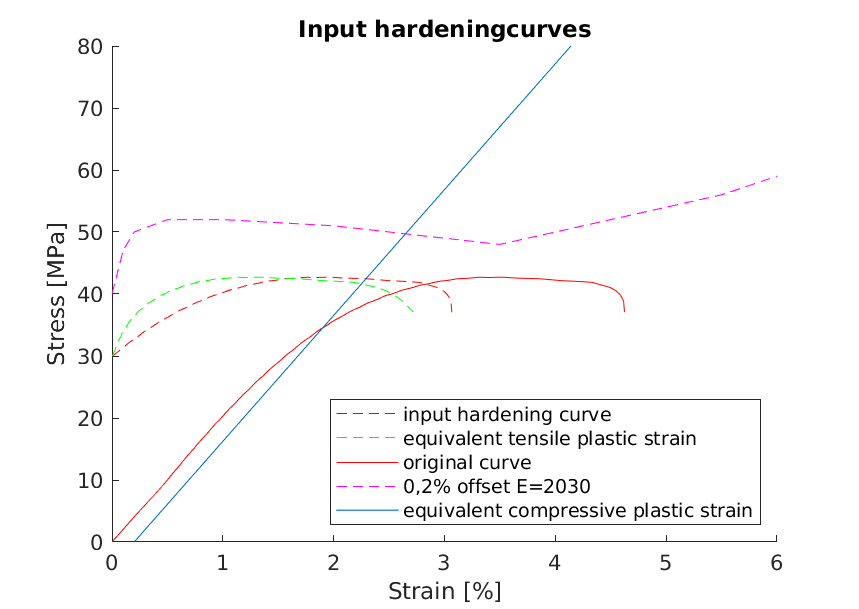
\includegraphics[width=0.60\textwidth]{chapter_7_non-elasticmodelling/figures/Hardening.png}
    \caption{Implemented hardening curves for Ultimaker ABS}
    \label{fig:hardening}
\end{figure}

The 0.2\% offset is used to indicate the yield point that would be defined for metals. The "anelastic" point (the point where linear elasticity practically ends and  where the hardening curve starts) is near this 0.2\% offset point. 

%explenation MATLAB code

Similar to the elastic modelling code, MATLAB is used to provide the input parameters and geometric shape. For the explicit method no periodic boundary conditions are applied, this would require too much computational power to run. In return, a convergence study is carried out for multiple stacked RVEs besides a convergence study for mesh sensitivity. 
%Load conditions. 
The mesh is loaded in the different loadcases, uniaxial tension in 1, 2 and 3 direction. The RVE is constrained on one face and loaded with a velocity boundary of equal to the $(a/20)/s$ where $a$ is the length of the parallel to the loading face. This results in a strain rate of around 1 mm/min, which is in accordance with the test speed used for the experimental investigation in chapter 5.
%Running the code
When the appropriate ABAQUS input files are generated by the MATLAB code, and the VUMAT file is defined alongside with the corresponding harderning curves, the job is submitted trough the unix shell to the kernel.
%Method of the code
For testing the constitutive model defined in the VUMAT a one element test was performed to asses the material response. The subroutines in VUMAT deterimes after every increment what the stress state is in the element, and what behaviour the element is coded to display. For the first region of the load, the element will behave elastically, up to the increment where the yield function defined by Tjoegbl (equation \ref{eqn:yieldpolymers}) is surpassed. At this moment the element behaves plastically and will follow the implemented hardening curve through an integration algorithm, which is described in more detail in Melro's paper \cite{Melro2013MicromechanicalModelling}.  Additionally the subroutine checks if the strain based Johnson Cook failure model is surpassed according to the defined Johnson Cook variation presented in equation \ref{eqn:JC}. This criterion implements an uniaxial tension strain to determine an equivalent strain that needs to be met before the element starts to fail. After this moment the element is deleted and will not exhibit any stiffness. 
In a larger model consisting of multiple elements, the geometry will create stress concentration points where elements will premature yield and fail. This will cause a crack to grow and finally will lead to fracture. The goal of the simulation is to determine the effect the geometry has on the macroscopic response of the RVE, that is, the reactional force opposite from the load face.
In a model consisting of multiple elements this subroutine is repeated for every element trough every increment. This RVE has more than 30000 elements and can go up to more than 300000 increments, resulting in running the subroutine more than $9*10^{10}$ times. This requires extensive computational power, therefore the High Performing Computing cluster of the TU Delft is used to perform this explicit analysis. Using the capabilities of one of the nodes in this computer, the simulation for each loading case took more than 4 hours in general.

The goal of the FEM simulation is to predict the stress strain response in the 3 principle directions and to compare these with the empirical tests. Additionally, different aspect ratios of the RVE as is discussed in chapter 4 can be simulated. But first a convergence study should be conducted to determine the accuracy of the simulations.
%mesh convergeance

When the FEM simulation finished, an ODB file is generated including the requested field and history output of certain time intervals. This includes i.a. the different types of stresses and strains etc. in the nodes and elements. The reaction forces (the amount of force a node "feels" when subjected to a load when it has no degrees of freedom) are prompted for the nodes. The nodes at the constrained face will generate enough information to determine the stress strain response of a certain load according to the following equation: 

\begin{equation} \label{eqn:RVESS}
1/A_{face}*\sum_{n=1} n_{face}
\end{equation}where $A_{face}$ is the surface of the constrained face and $n_{face}$ are the nodes at the constrained face. 

\subsection{Convergence study}
To determine the mesh sensitivity a convergence study is conducted. The same meshing strategy, including the partitioning, was implemented as is presented in chapter 6. Element sizes of 0.004 0.006 0.008 and 0.01 mm are tested for the 3 directions for an aspect ratio of 0.5. The different forms of meshes are presented in figure \ref{fig:meshes}. The results of these meshes are found in figure \ref{fig:meshconv}. However, these meshes did not seem to converge, which complicated things. Especially since the ratio between element size and porosity for the lower aspect ratio's would only increase, resulting in a even larger difference.  Additionally, the computational resources for the 0.004 mesh were already quite expensive, needing +30 hours CPU time for 1 simulation. Therefore, a different strategy was used. First, multiple CPU's were used for the following simulations, 8 CPU's seemed the optimal amount for hyper threading Abaqus Explicit jobs. Secondly, mass scaling was applied to increase the Stable Time Increment. After some experimentation, mass scaling of 27.5 was applied to increase the Stable Time Increment of the smallest elements from $2*10^{-7}$ to $1*10^{-6}$. Higher mass scaling introduces a too much kinetic energy, which in turn generated stress waves in the stress strain curves, which is highly undesirable. Finally, the mesh strategy was adjusted. The goal was to still implement hexahedrals, due to their symmetry and favourable geometry, but to decrease the density in the area's without stress concentrations. The new strategy resulted in seeding the edges of the cavity with a fine mesh, while the rest of the RVE is meshed with a coarse 0.01 mesh as can be seen in figure \ref{fig:meshopt}. This mesh will be referred to as "optimized mesh", and reduced the number of elements with a factor 10 (from $4*10^6$ to $4*10^5$ elements). With these measures the computational time has been decreased with approximately factor  400. The current simulations are often finished in 8 hours. 

\begin{figure}
\centering
  \begin{subfigure}[b]{0.48\textwidth}
    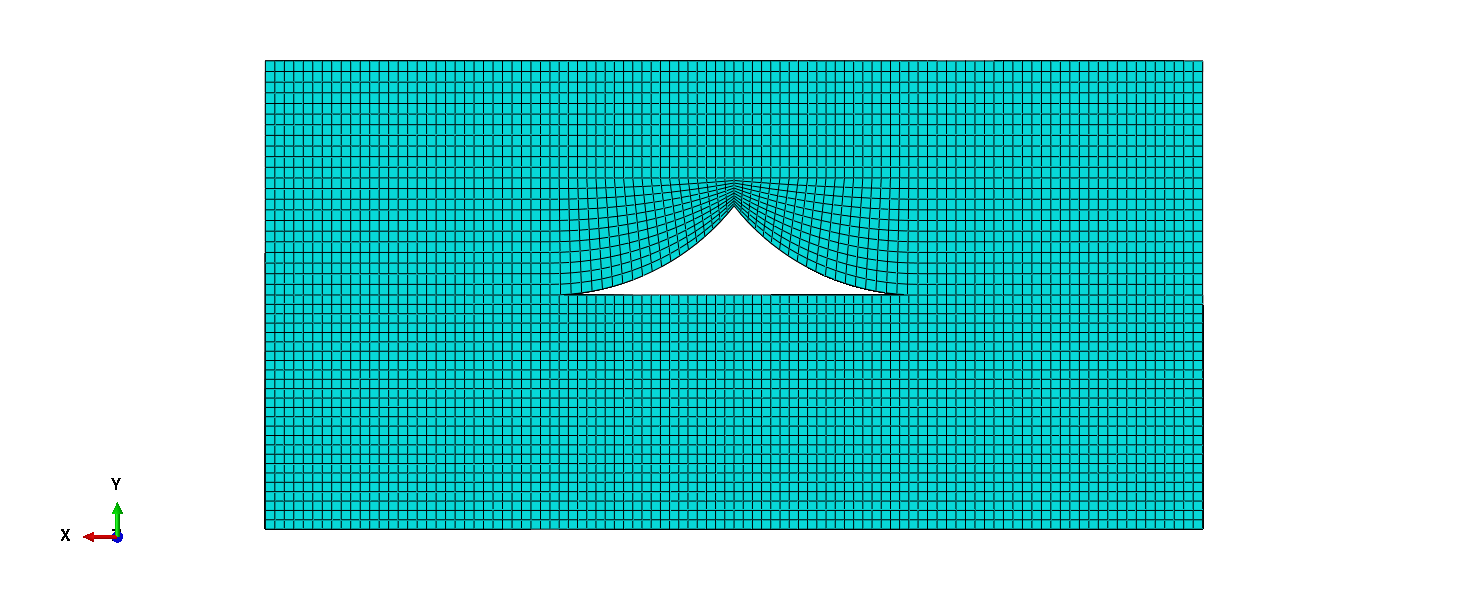
\includegraphics[width=\textwidth]{chapter_7_non-elasticmodelling/figures/mesh0004.png}
    \caption{ mesh 0.004}
  \end{subfigure}
  %
  \begin{subfigure}[b]{0.48\textwidth}
    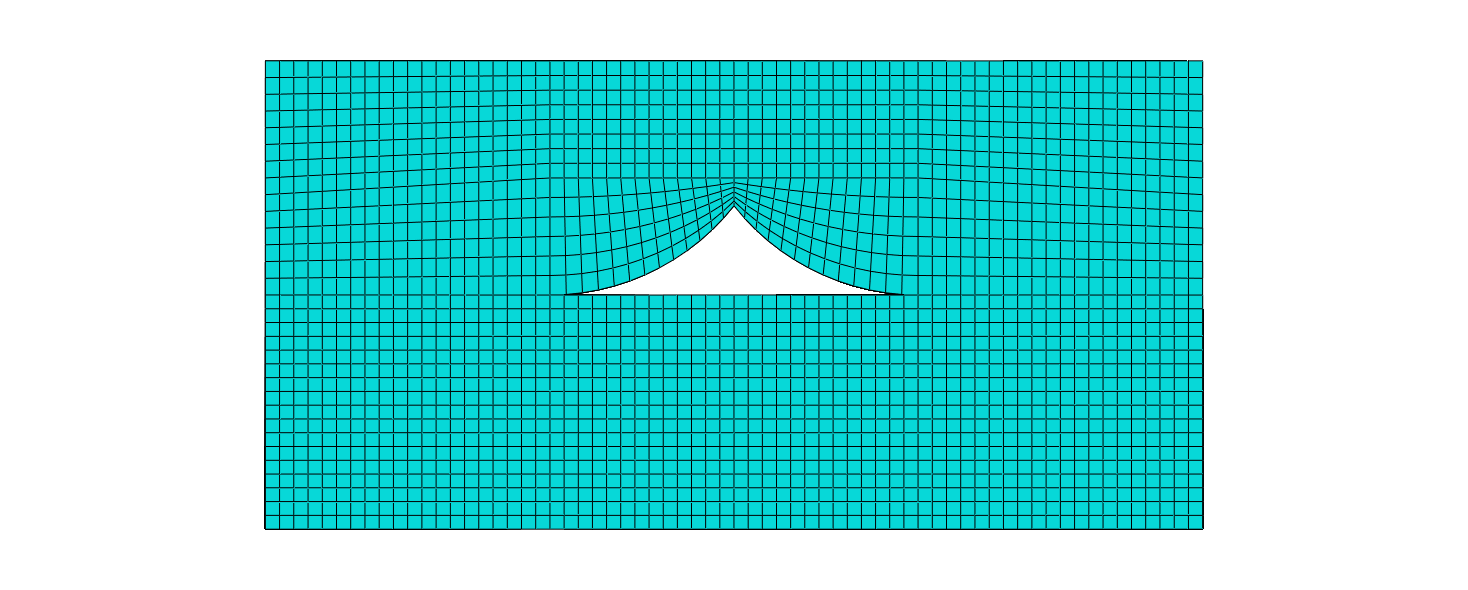
\includegraphics[width=\textwidth]{chapter_7_non-elasticmodelling/figures/mesh0006.png}
    \caption{ mesh 0.006}
  \end{subfigure}
  \\
    \begin{subfigure}[b]{0.48\textwidth}
    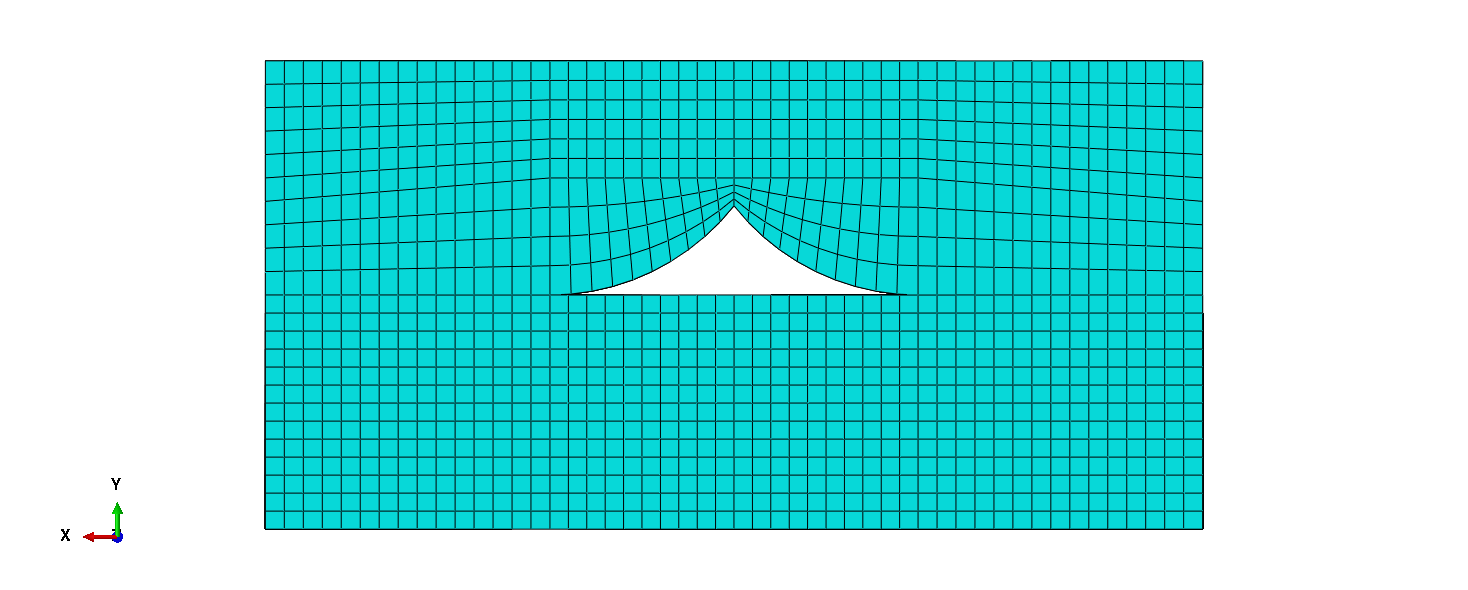
\includegraphics[width=\textwidth]{chapter_7_non-elasticmodelling/figures/mesh0008.png}
    \caption{ mesh 0.008}
  \end{subfigure}
  %
  \begin{subfigure}[b]{0.48\textwidth}
    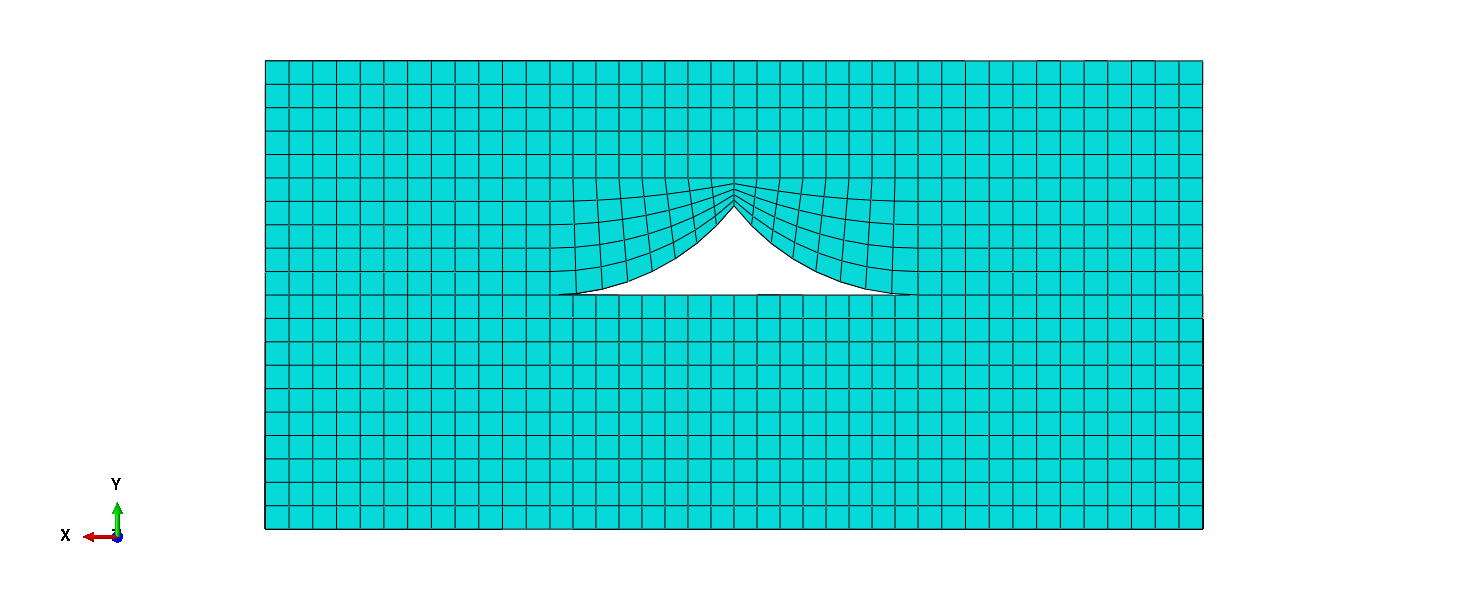
\includegraphics[width=\textwidth]{chapter_7_non-elasticmodelling/figures/mesh001.png}
    \caption{ mesh 0.01}
  \end{subfigure}
  \\
  
  \caption{Different element sizes implemented for convergence study.}
  \label{fig:meshes}
\end{figure}
\begin{figure}[H]
    \centering
    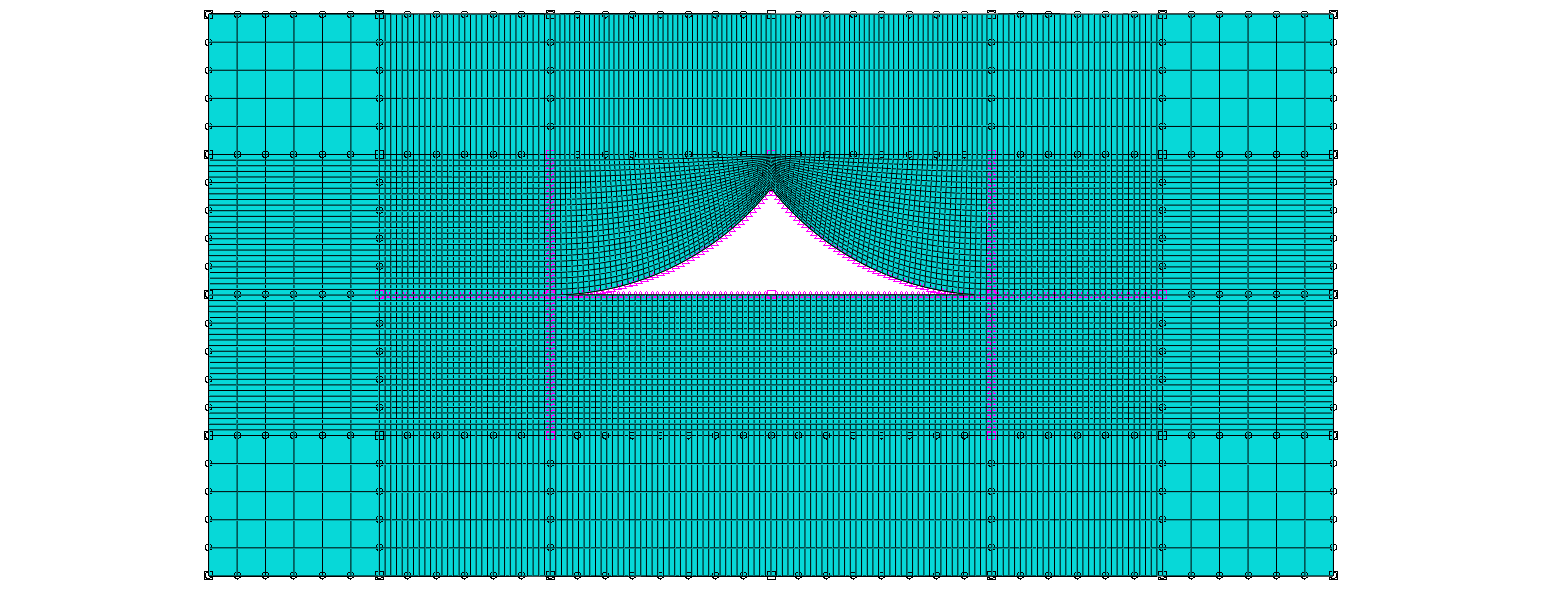
\includegraphics[width=0.60\textwidth]{chapter_7_non-elasticmodelling/figures/meshopt.png}
    \caption{Optimized mesh with a fine node seed (0.002) along the cavity and coarse (0.01) for the rest.}
    \label{fig:meshopt}
\end{figure}

Additionally, a convergence study is conducted for multiple connected RVEs. Four stacked RVEs in the XY and ZX planes are analyzed and additionally a block of 2 x 2 x 2 RVEs is simulated. The RVEs are produced with a aspect ratio of 0.5 and with an element size of 0.01, similar to the generation of the RVE for the elastic analysis. The RVE combinations can be seen in figure \ref{fig:mulRVE}.

\begin{figure}
\centering
  \begin{subfigure}[b]{0.48\textwidth}
    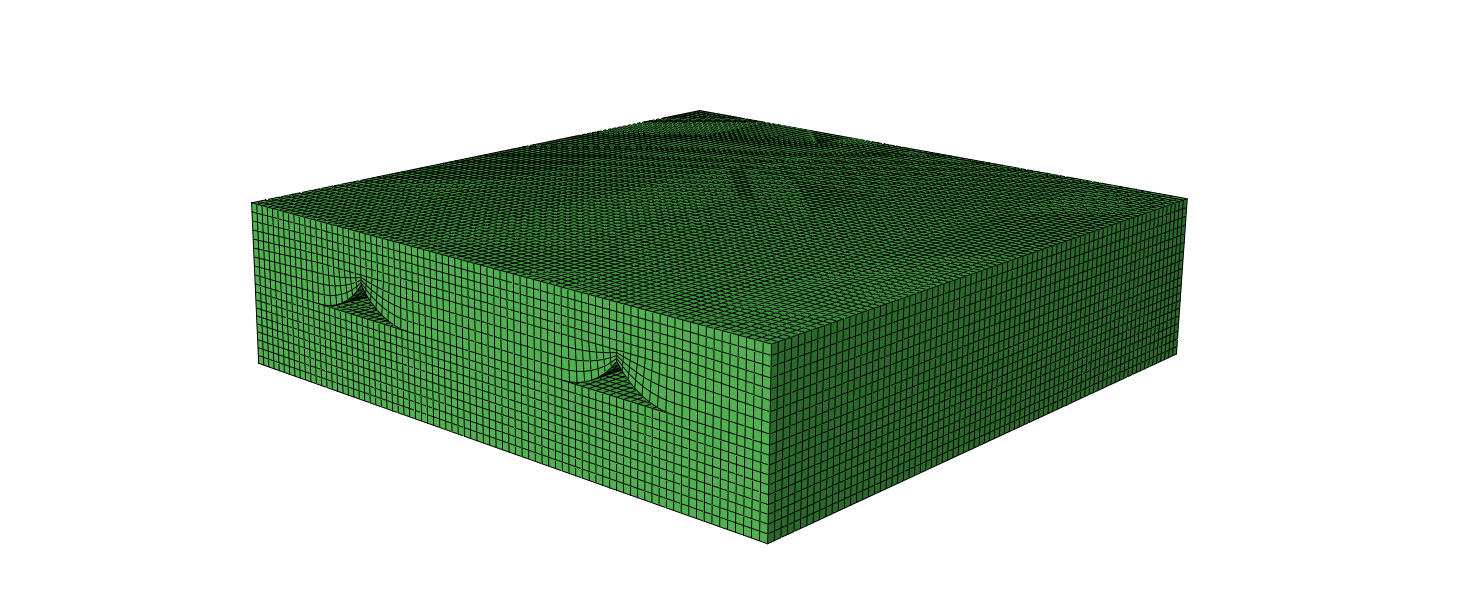
\includegraphics[width=\textwidth]{chapter_7_non-elasticmodelling/figures/RVEXY.png}
    \caption{ RVE XY plane}
  \end{subfigure}
  %
  \begin{subfigure}[b]{0.48\textwidth}
    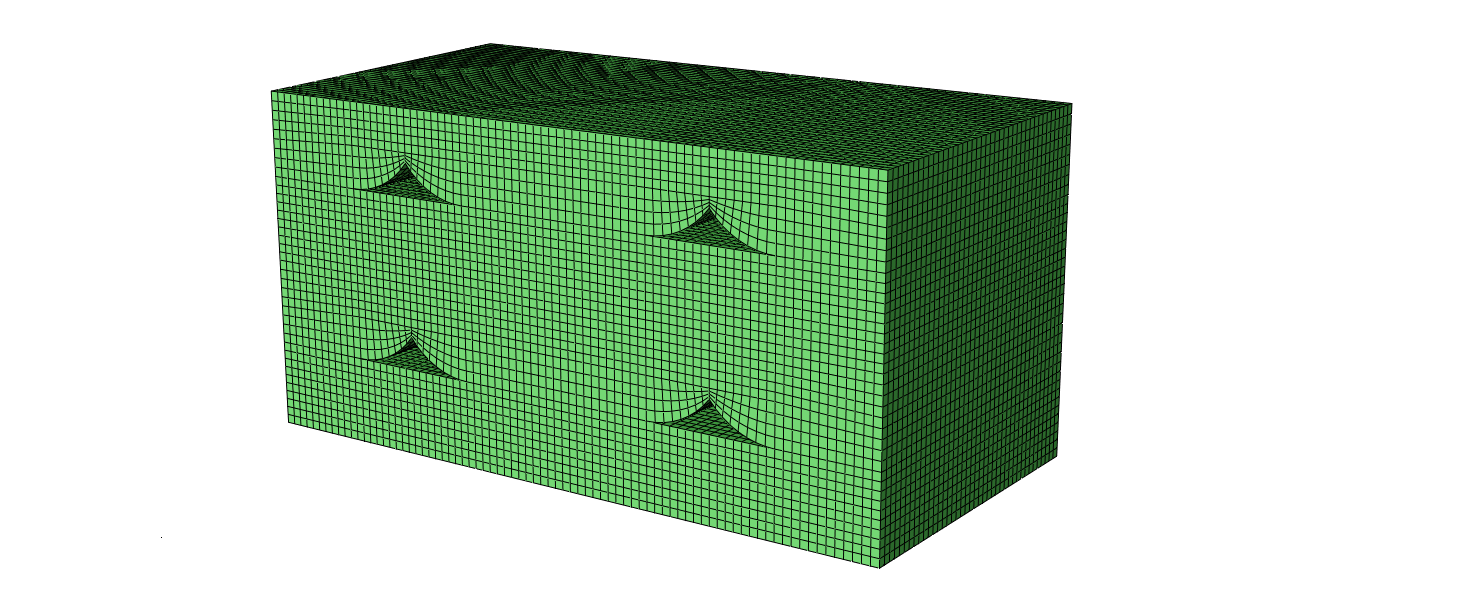
\includegraphics[width=\textwidth]{chapter_7_non-elasticmodelling/figures/RVEZX.png}
    \caption{ RVE ZX plane}
  \end{subfigure}
  \\
    \begin{subfigure}[b]{0.48\textwidth}
    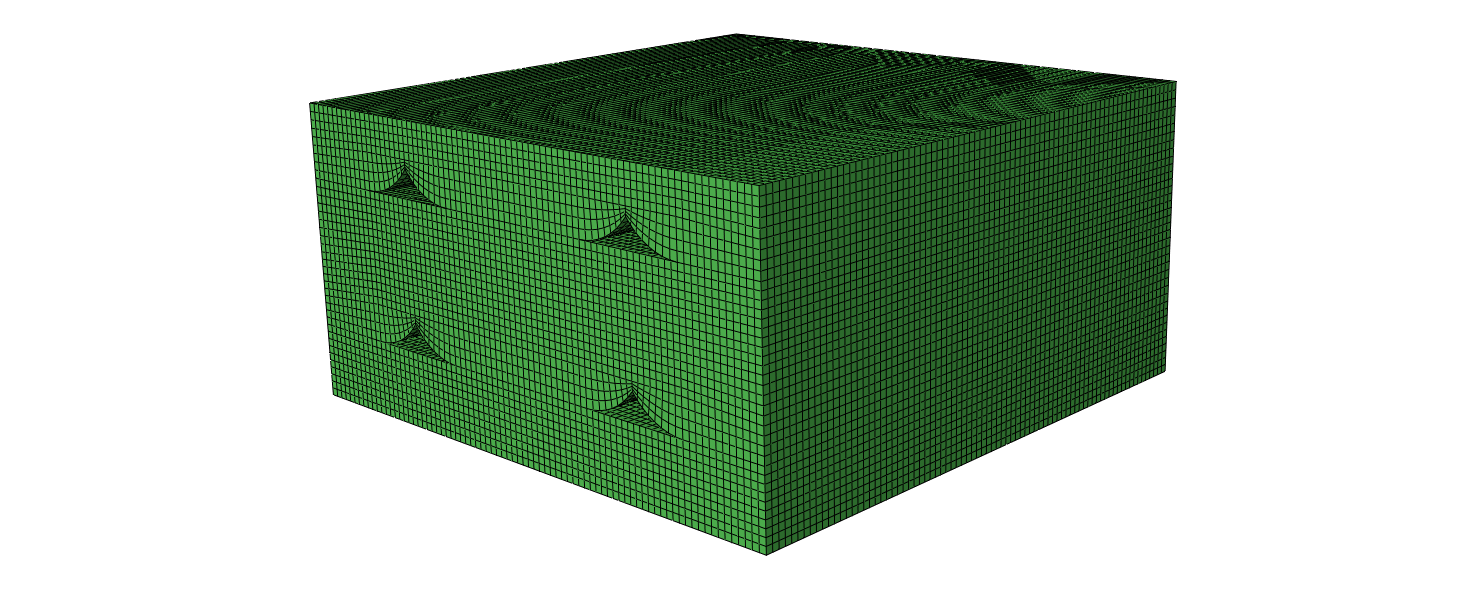
\includegraphics[width=\textwidth]{chapter_7_non-elasticmodelling/figures/RVEZYX.png}
    \caption{ RVE ZYX direction }
  \end{subfigure}
  %
  
  \caption{Different RVE duplicates implemented for convergence study.}
  \label{fig:mulRVE}
\end{figure}

\subsection{Stress Intensity approach}
An additional approach was investigated with respect to the failure mechanism in the RVE. As is described in chapter 2, linear elastic fracture mechanics states that the critical failure stress can be predicted if the form and size of a crack is known. The equation for the stress intensity factor can be seen in equation \ref{eqn:criticalstress}. The periodic voids can be assumed as cracks for a plane strain loading condition in the 2 and 3 direction, which are dependant on the line thickness and width. With these parameters a critical stress $(\sigma_c)$ can be found which should give an approximation for the failure stress in FFF produced parts.  The the fracture toughness of ABS, a $K_{Ic}$ of 

Additionally, the cracktip plasticity theory, explained in chapter 2 (\ref{eqn:cracktip}) is used to predict the radius of the plastic deformation. This is useful to predict the plastic behaviour involved in the failure of parts. Products that show low plasticity in their fracture surface are suspected to have a low toughness at the fracture surface, resulting in brittle failure, which might be caused by improper failure. To have a better understanding of the size of the cracktip plasitcity, the radius of plasticity is plotted against the distance between the crack tip and the edge of the RVE. These lengths are not equal in the 3 direction, therefore the average of both lengths is used to determine the distance between two cavities. 

\section{Results}
\subsection{Convergence study mesh}
The convergence study of the mesh for mesh sizes 0.004, 0.006, 0.008 and 0.01 with an RVE with aspect ration 0.5 is presented in figure \ref{fig:meshconv}. The 3 principal directions are presented consecutively in green, red and blue. For some mesh sizes the simulations were unsuccessfully (0.004 in 1 and 2 direction and 0.006 in 1 direction), the simulations in the 3 direction give a representative view on the mesh sensitivity.  As can be seen,  convergence is difficult to achieve due to the large stress concentrations at the tips of the cavity, the difference between 0.004 mm and 0.002 mm is still significant. It is however very difficult, and computationally expensive to decrease the mesh even further.  

\begin{figure}[H]
    \centering
    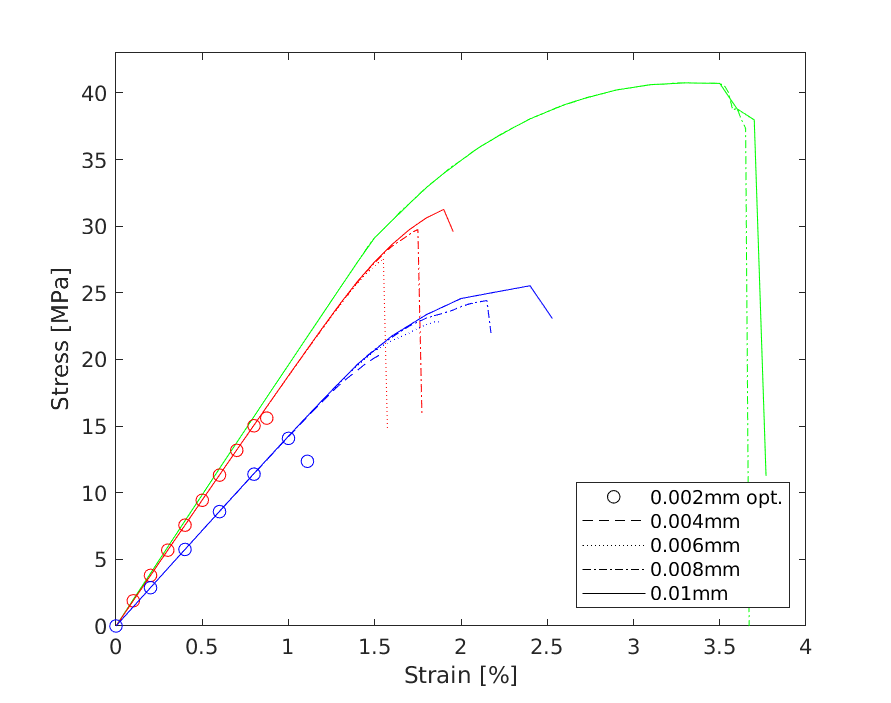
\includegraphics[width=0.60\textwidth]{chapter_7_non-elasticmodelling/figures/meshconv.png}
    \caption{Convergence study for different mesh sizes}
    \label{fig:meshconv}
\end{figure}

\subsection{Convergence study RVEs}
The convergence study for the RVE duplicates are presented in figure \ref{fig:RVEgraph}, and are related to the figures is figure \ref{fig:mulRVE}. Here the ZYX RVE in the 1 principal direction failed, the other results give a good representation of the sensitivity of the multiple RVEs. As can be seen, the difference in response is minimal for different RVE stacks. 

\begin{figure}[H]
    \centering
    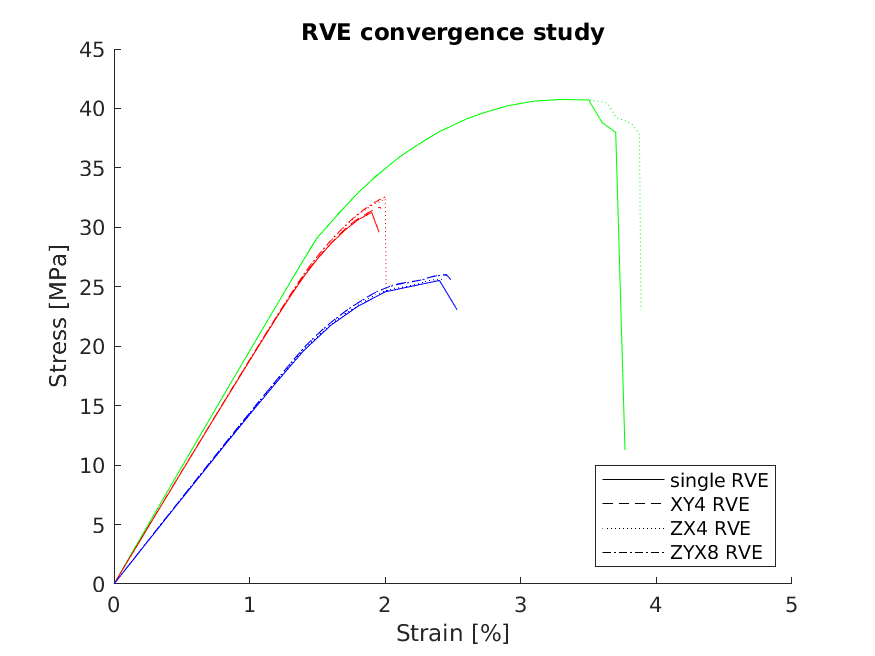
\includegraphics[width=0.60\textwidth]{chapter_7_non-elasticmodelling/figures/RVEconv.png}
    \caption{Convergence study for RVE duplicates}
    \label{fig:RVEgraph}
\end{figure}

\subsection{Simulations compared with empirical results }
In figure \ref{fig:ComparisonSS} the 0.5 aspect ratio simulation with the optimized mesh is compared with the empirical results from the 0.4 x 0.2 ASTM 3039 tensile test samples presented in chapter 5. The results between the empirically measured and simulated RVE show significant overlap, with the 1 and 2 direction showing 10\% difference in the UTS. Elongation at break is very accurately predicted for the 2 direction, with a difference of 6\%, the 1 direction has a difference of 25\%. The 3 direction is less accurate for the UTS and elongation at break, but the ASTM curve still overlaps the simulated RVE. This will further be explained in the discussion.

\begin{figure}[H]
    \centering
    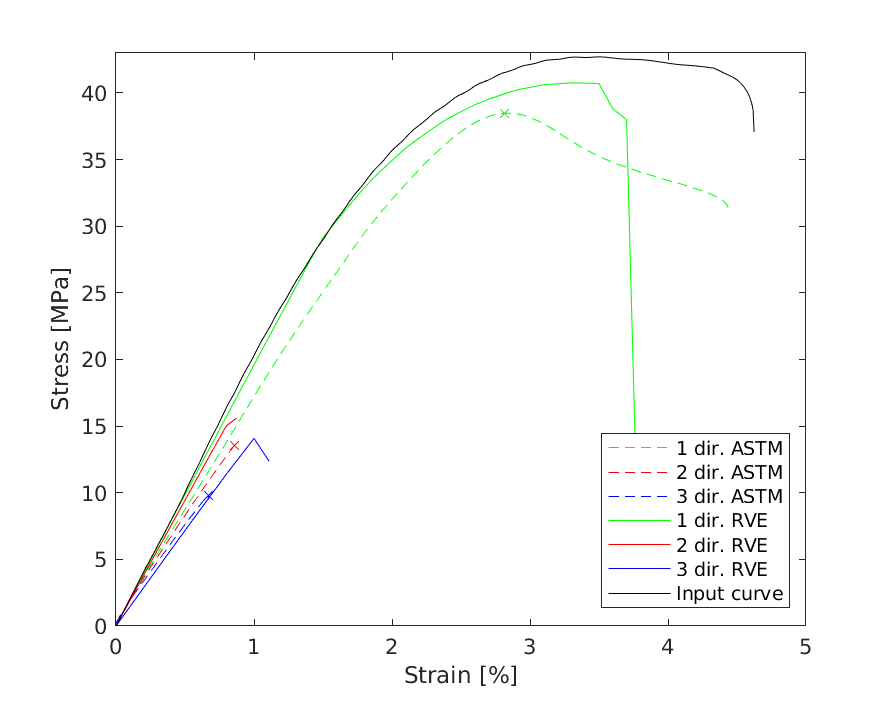
\includegraphics[width=0.60\textwidth]{chapter_7_non-elasticmodelling/figures/ComparisonSS.png}
    \caption{Comparison between the empirical obtained results and the simulated RVE in the 3 principle directions}
    \label{fig:ComparisonSS}
\end{figure}

\subsection{Simulations with altering aspect ratio}
In the following figures ( \ref{fig:AR1},\ref{fig:AR2},\ref{fig:AR2} ) the dependency on the aspect ratio is shown for the optimized mesh. Aspect ratios of 0.125, 0.2, 0.25, 0.5, 0.75 and 1 are simulated for the 3 principle directions. 

\begin{figure}[H]
    \centering
    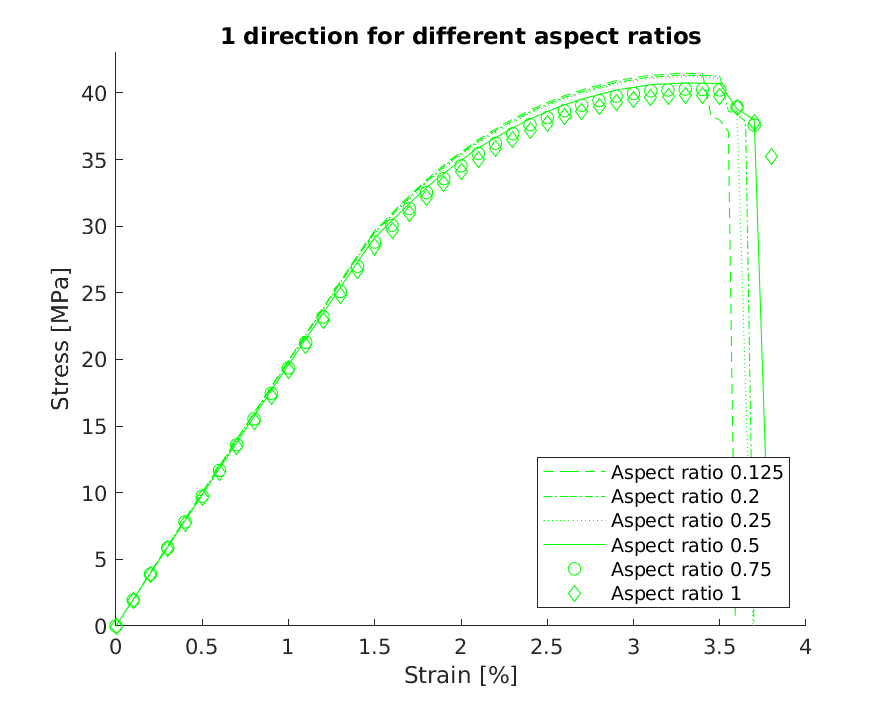
\includegraphics[width=0.60\textwidth]{chapter_7_non-elasticmodelling/figures/AR1.png}
    \caption{Comparison between different aspect ratios in the 1 direction}
    \label{fig:AR1}
\end{figure}
\begin{figure}[H]
    \centering
    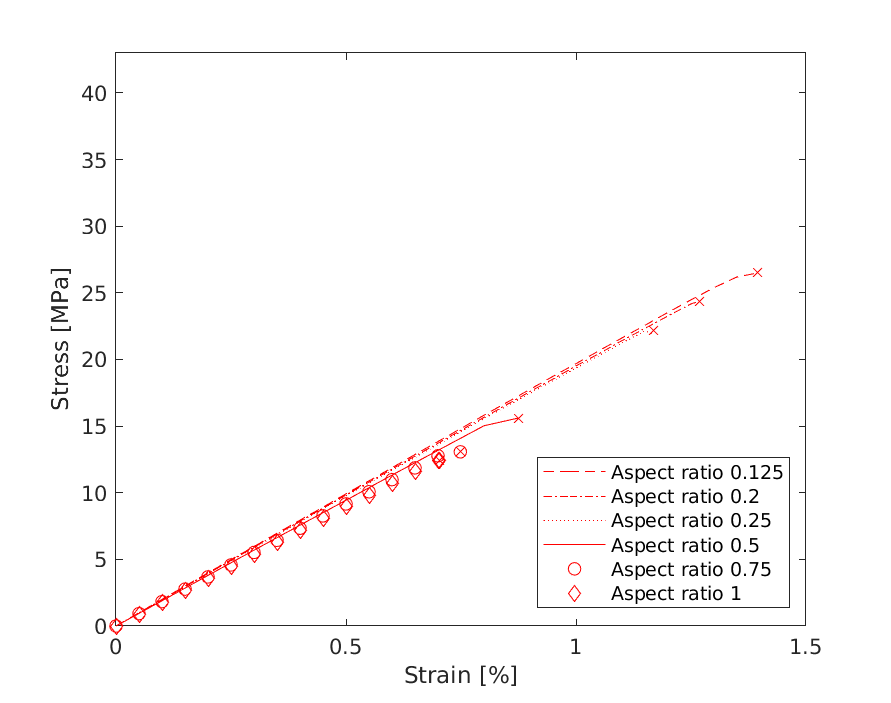
\includegraphics[width=0.60\textwidth]{chapter_7_non-elasticmodelling/figures/AR2.png}
    \caption{Comparison between different aspect ratios in the 2 direction}
    \label{fig:AR2}
\end{figure}
\begin{figure}[H]
    \centering
    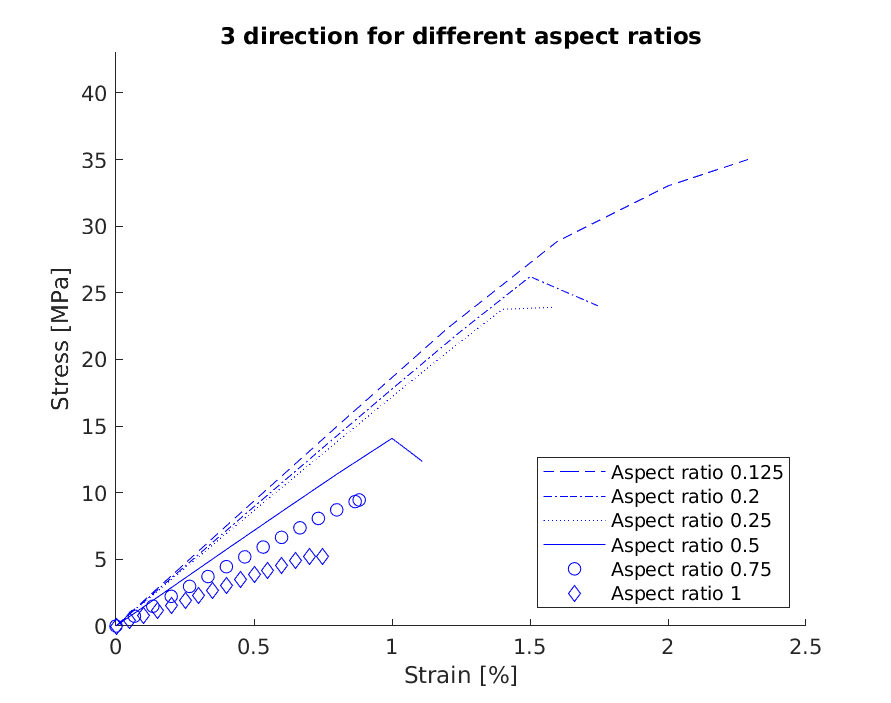
\includegraphics[width=0.60\textwidth]{chapter_7_non-elasticmodelling/figures/AR3.png}
    \caption{Comparison between different aspect ratios in the 3 direction}
    \label{fig:AR3}
\end{figure}
\subsection{Contour plots of different aspect ratios }
The following figures (\ref{fig:Contourplot} will present the contour plots at the moment before failure of the maximum equivalent total strain of the 3 principal directions for the aspect ratios of 0.125, 0.5 and 1. Since the Johnson Cook model is implemented based on a equivalent total strain of 0.0606 in tensile, this will give a decent representation of the region of failure. Note that the Johnson Cook criterion is dependant on the stress triaxiality, this means that the equivalent total strain at fracture can be higher or lower than the implemented uni-axial fracture strain of 0.0606 for complex strain states.

\begin{figure}
\centering
  \begin{subfigure}[b]{0.6\textwidth}
    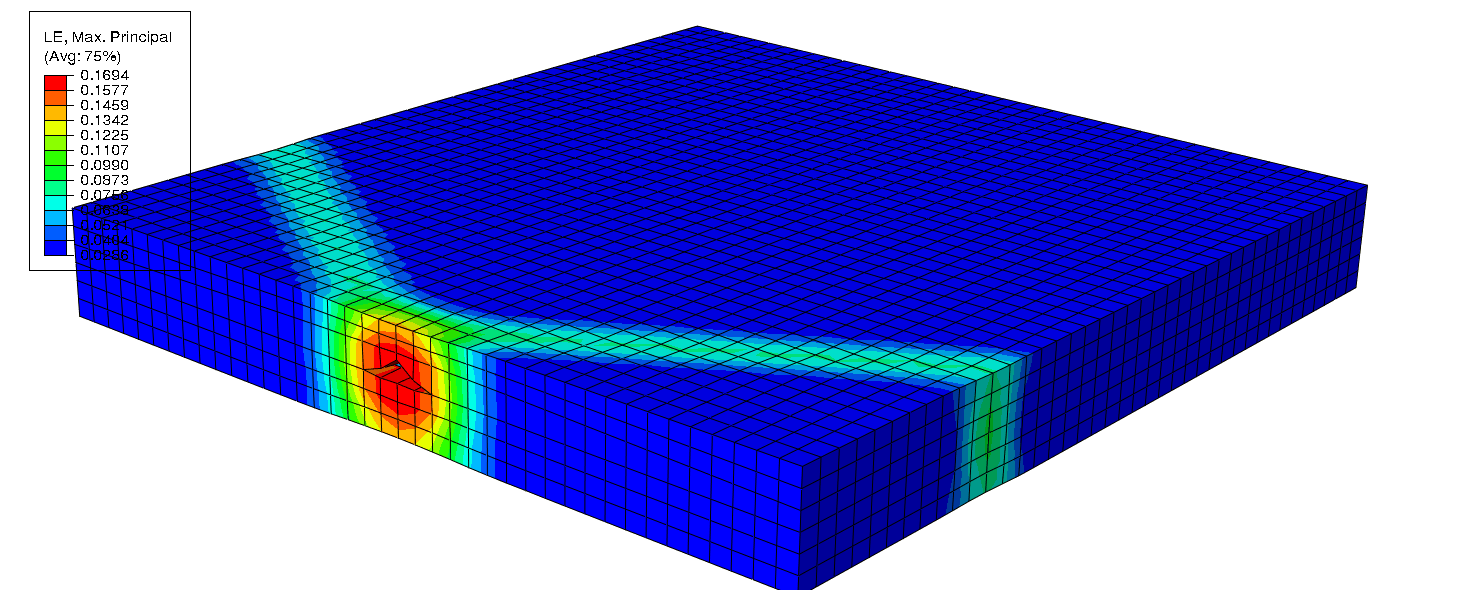
\includegraphics[width=\textwidth]{chapter_7_non-elasticmodelling/figures/0125p1.png}
    \caption{0.125 aspect ratio, 1 direction}
  \end{subfigure}
  \\
  \begin{subfigure}[b]{0.6\textwidth}
    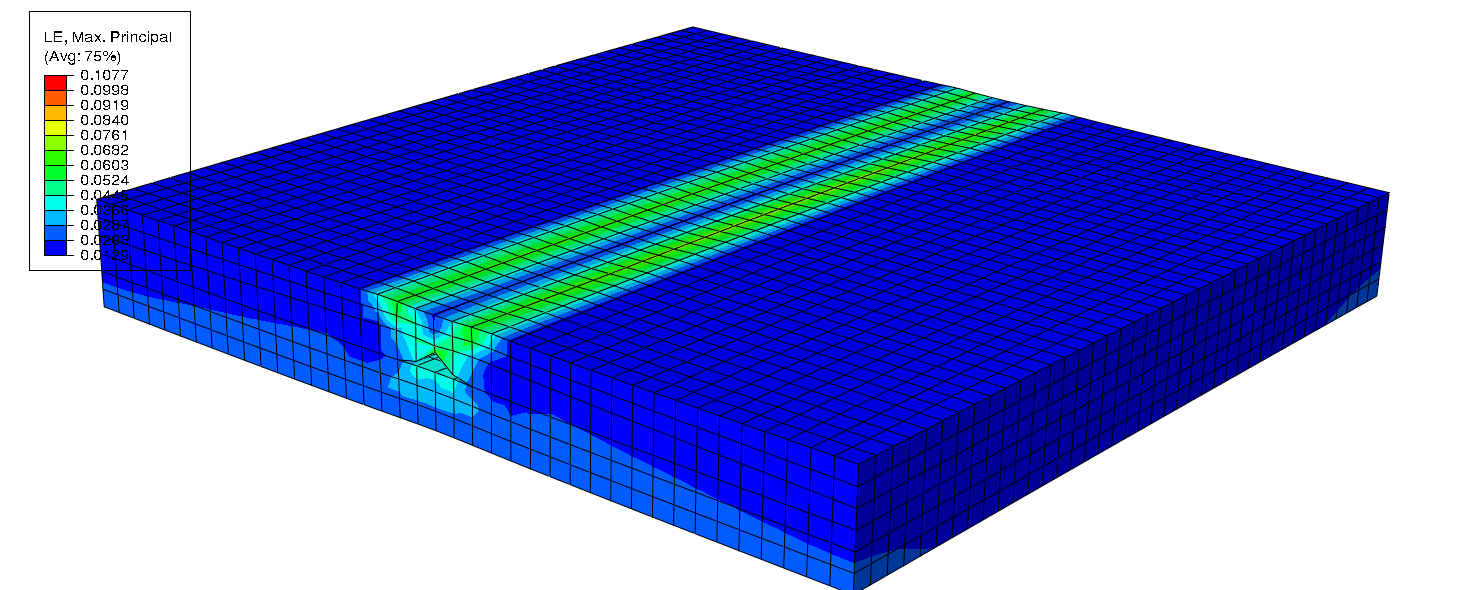
\includegraphics[width=\textwidth]{chapter_7_non-elasticmodelling/figures/0125p2.png}
    \caption{0.125 aspect ratio, 2 direction}
  \end{subfigure}
  \\
    \begin{subfigure}[b]{0.60\textwidth}
    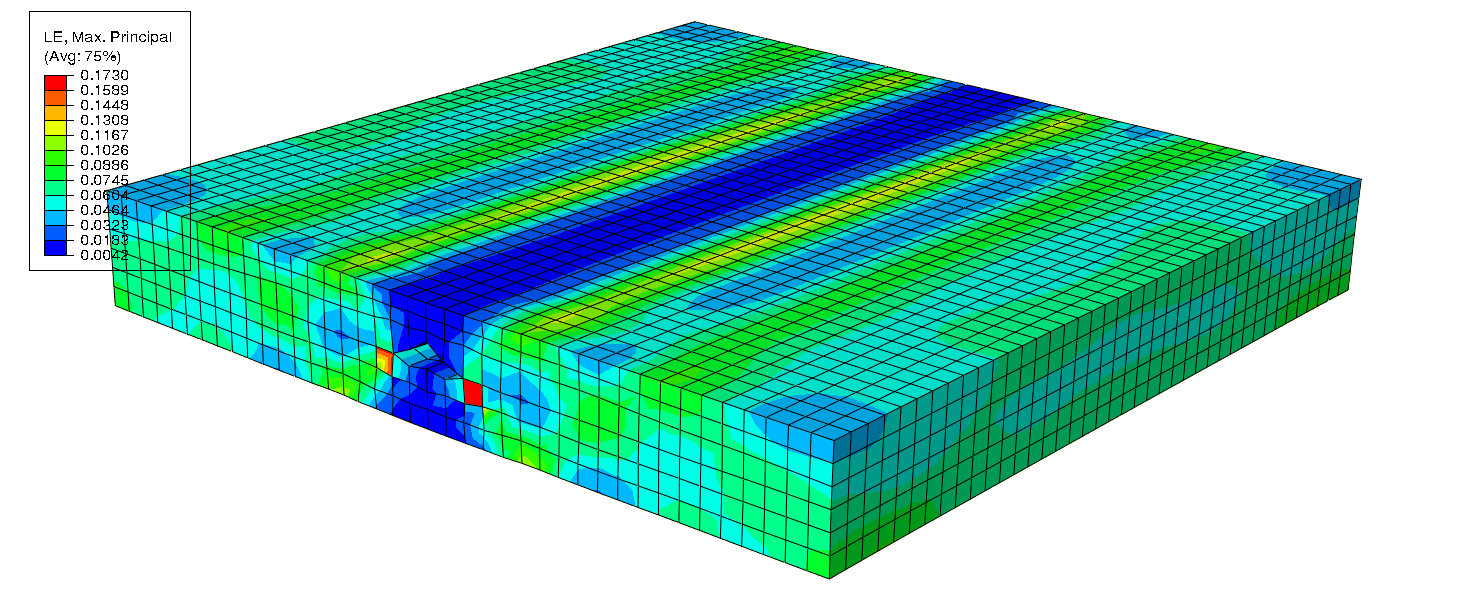
\includegraphics[width=\textwidth]{chapter_7_non-elasticmodelling/figures/0125p3.png}
    \caption{0.125 aspect ratio, 3 direction}
  \end{subfigure}
  \\
  \begin{subfigure}[b]{0.70\textwidth}
    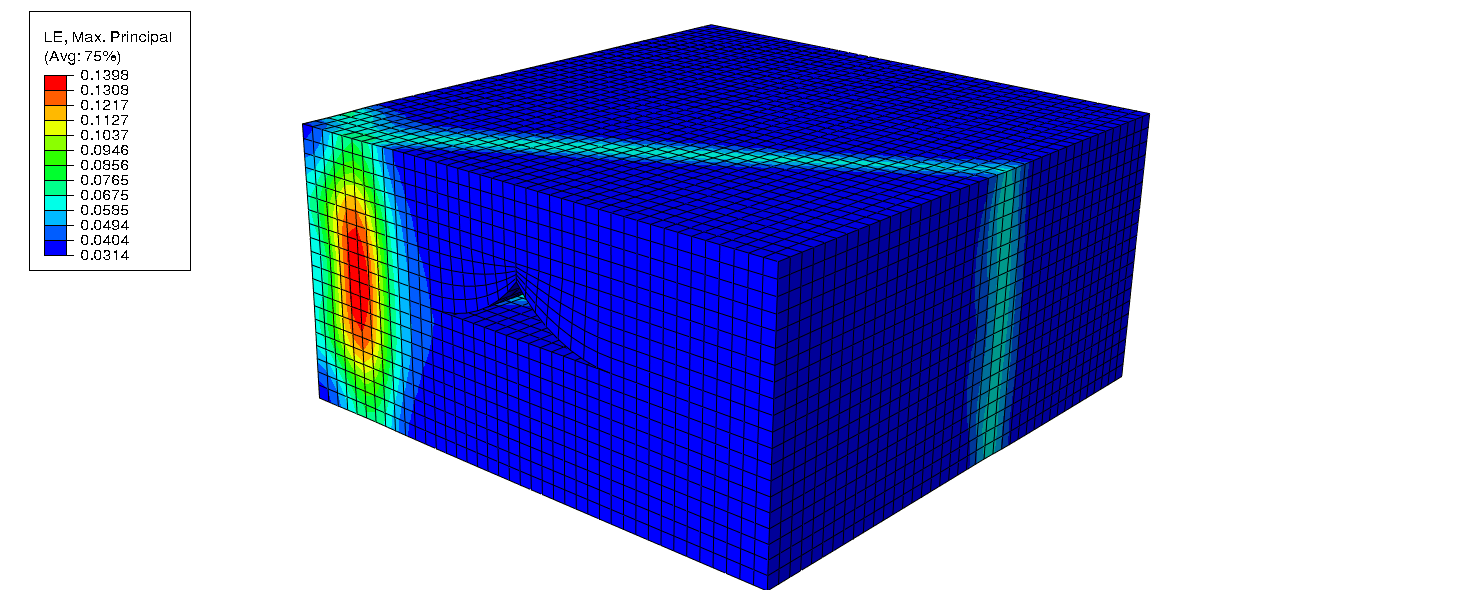
\includegraphics[width=\textwidth]{chapter_7_non-elasticmodelling/figures/05p1.png}
    \caption{0.5 aspect ratio, 1 direction}
  \end{subfigure}
  \\
    \begin{subfigure}[b]{0.70\textwidth}
    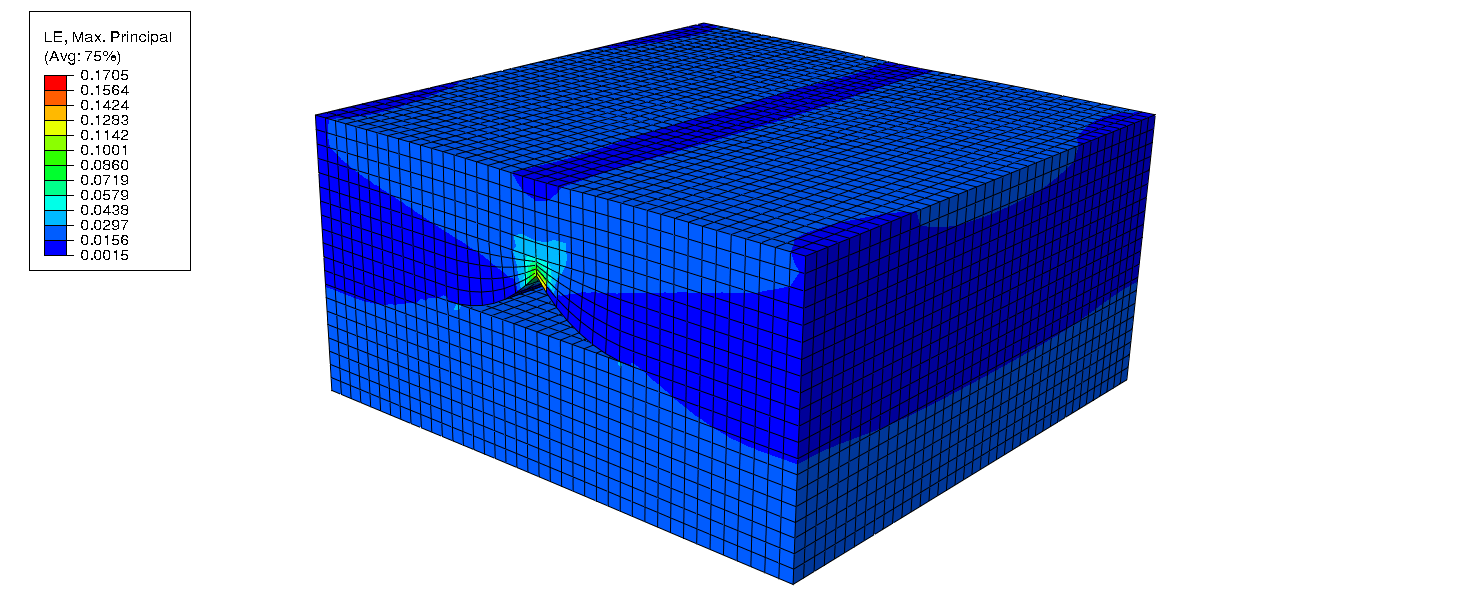
\includegraphics[width=\textwidth]{chapter_7_non-elasticmodelling/figures/05p2.png}
    \caption{0.5 aspect ratio, 2 direction}
  \end{subfigure}
  \end{figure}
  \\
  \begin{subfigure}[b]{0.70\textwidth}
    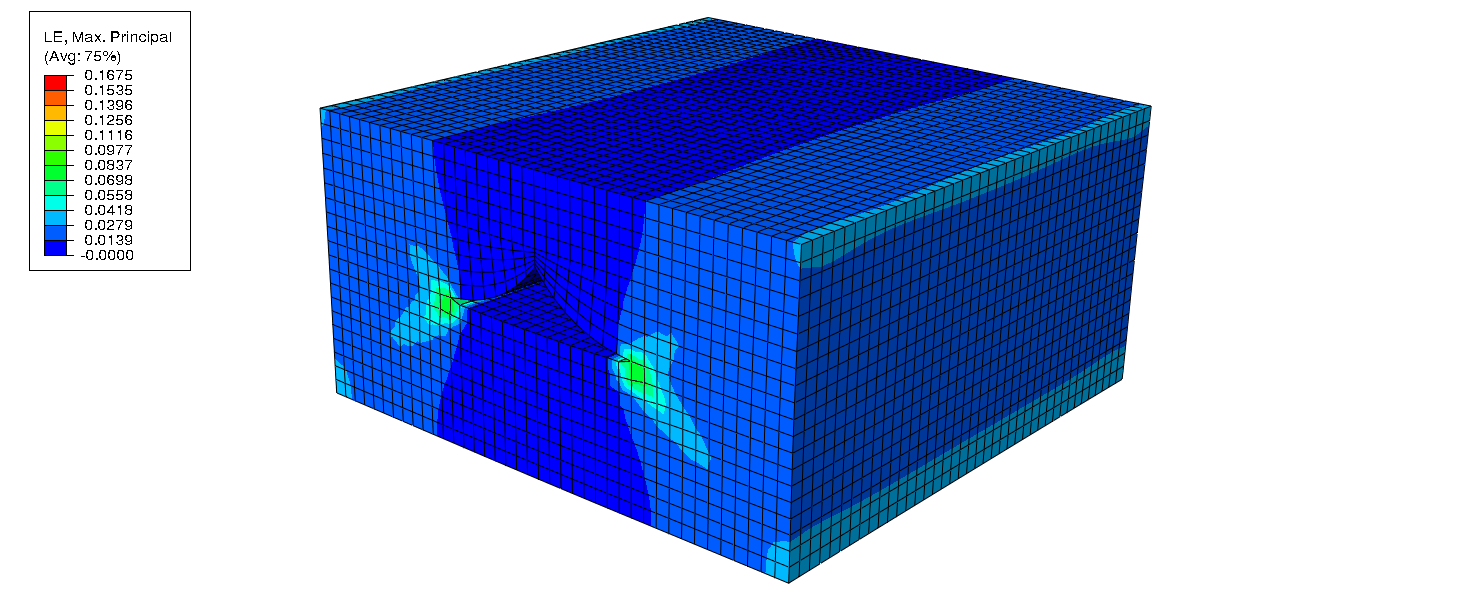
\includegraphics[width=\textwidth]{chapter_7_non-elasticmodelling/figures/05p3.png}
    \caption{0.5 aspect ratio, 3 direction}
  \end{subfigure}
  \\
    \begin{subfigure}[b]{0.80\textwidth}
    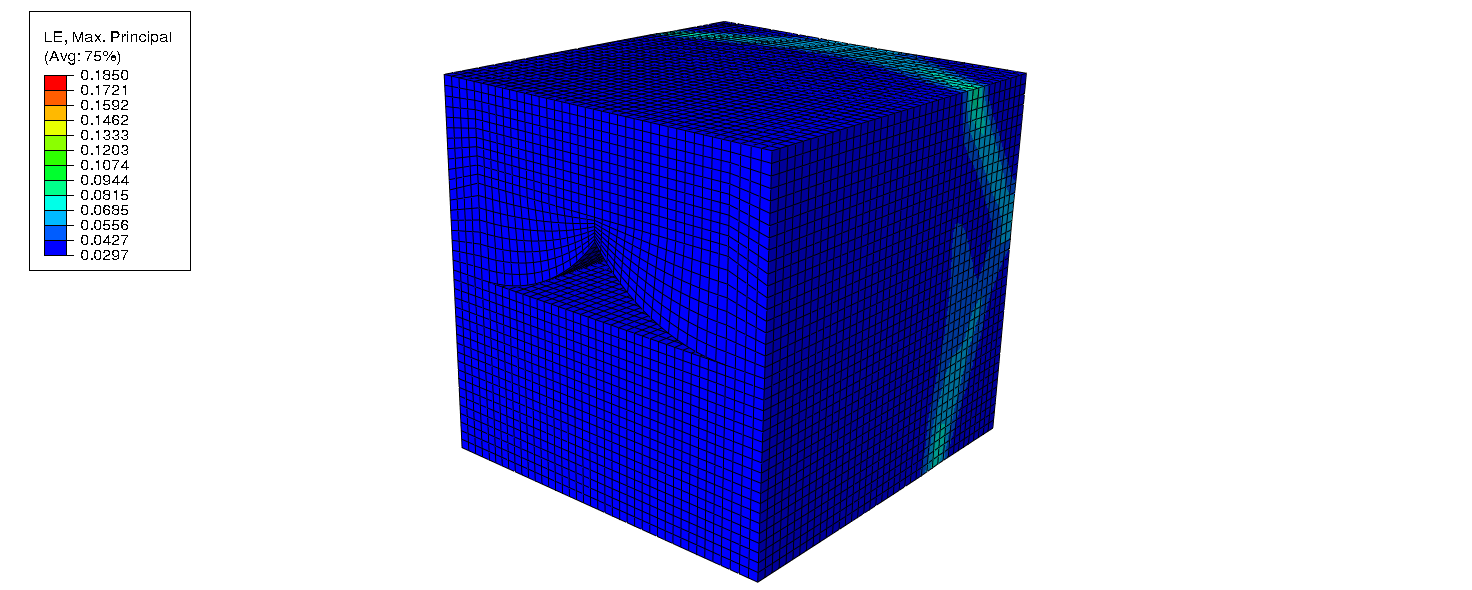
\includegraphics[width=\textwidth]{chapter_7_non-elasticmodelling/figures/1p1.png}
    \caption{1 aspect ratio, 1 direction}
  \end{subfigure}
  \\
    \begin{subfigure}[b]{0.80\textwidth}
    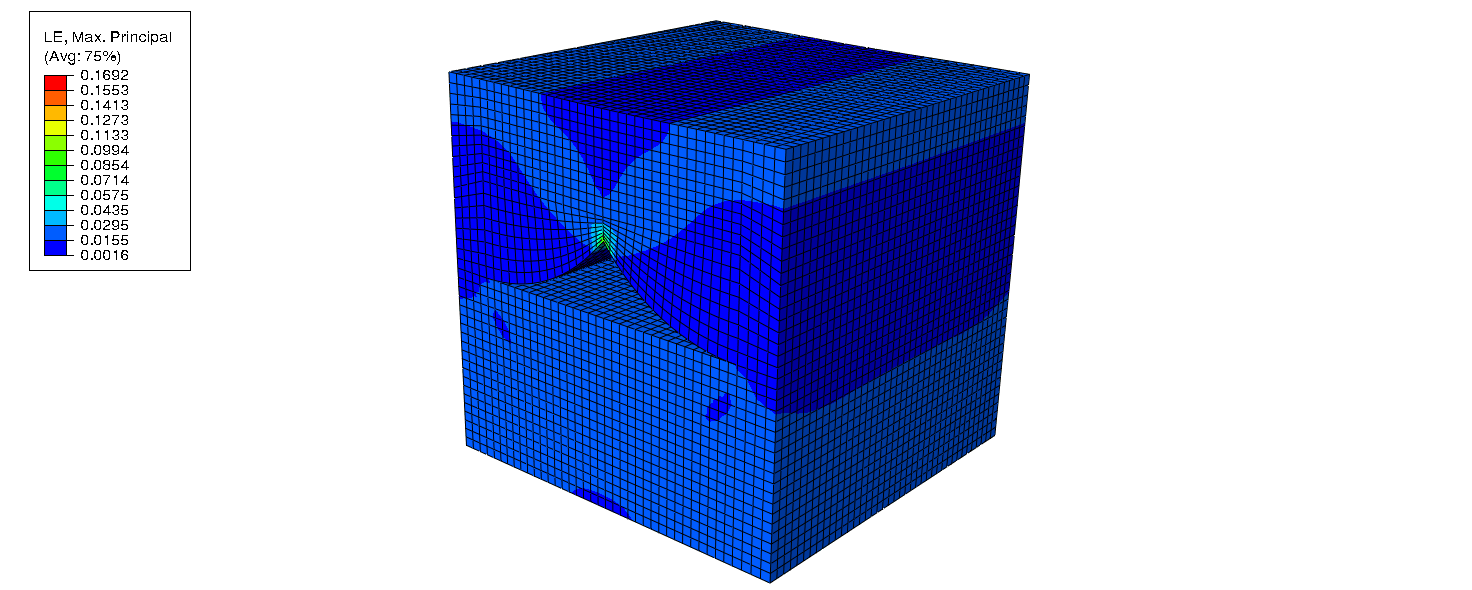
\includegraphics[width=\textwidth]{chapter_7_non-elasticmodelling/figures/1p2.png}
    \caption{1 aspect ratio, 2 direction}
  \end{subfigure}
  \\
  \begin{subfigure}[b]{0.80\textwidth}
    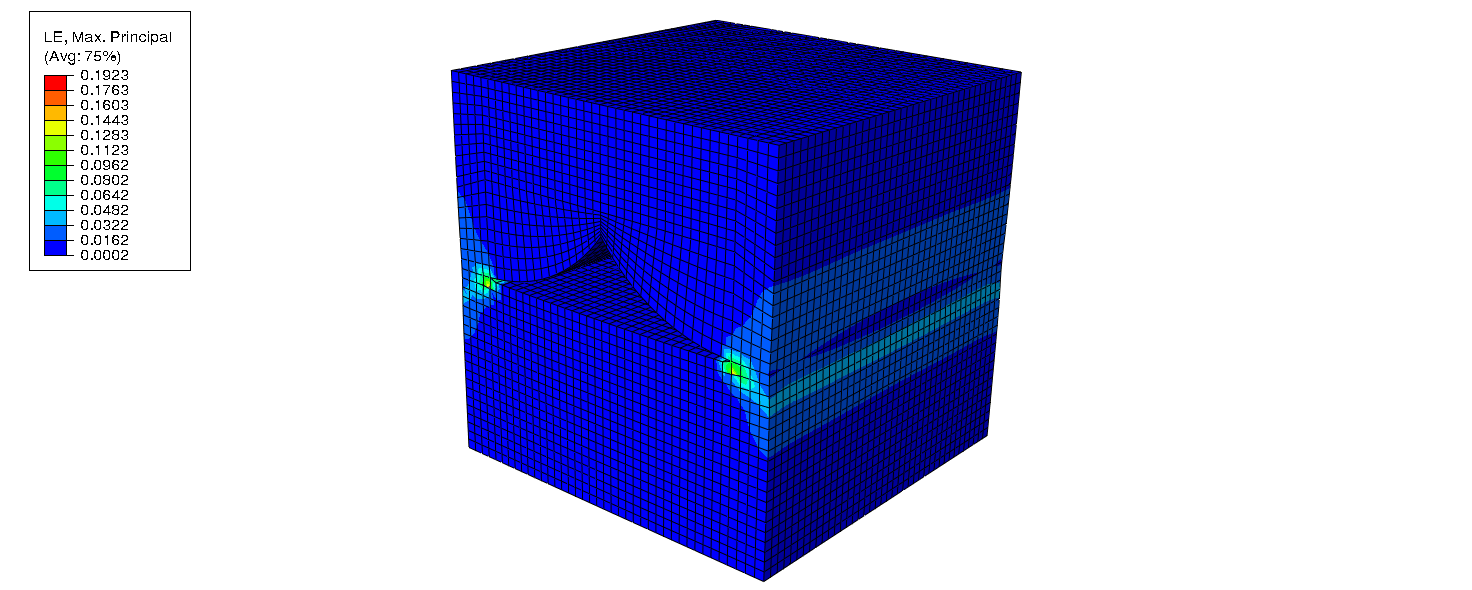
\includegraphics[width=\textwidth]{chapter_7_non-elasticmodelling/figures/1p3.png}
    \caption{1 aspect ratio, 3 direction}
  \end{subfigure}
  \caption{Contour plots of different aspect ratios just before failure}
  \label{fig:Contourplot}
\end{figure}

\subsection{Comparison fracture stress}
In figure \ref{fig:fracturestress} the plots (according to equation of critical stress in fracture mechanics \ref{eqn:criticalstress} and the Rule of Mixture \ref{eqn:ROM}) and simulated fracture stresses are presented and compared along different aspect ratios. The 1 direction is predicted with a plot of the Rule of Mixtures, while the 2 and the 3 directions are predicted with the plot of the critical stress equation. The Rule of mixtures overestimates the fractures stress with about 5\%. 
When looking at the 2 and 3 directions, one can see the similarity of the inverse exponential behaviour between the plotted results from the equation and simulated datapoints. 

%wait with wr

\begin{figure}[H]
    \centering
    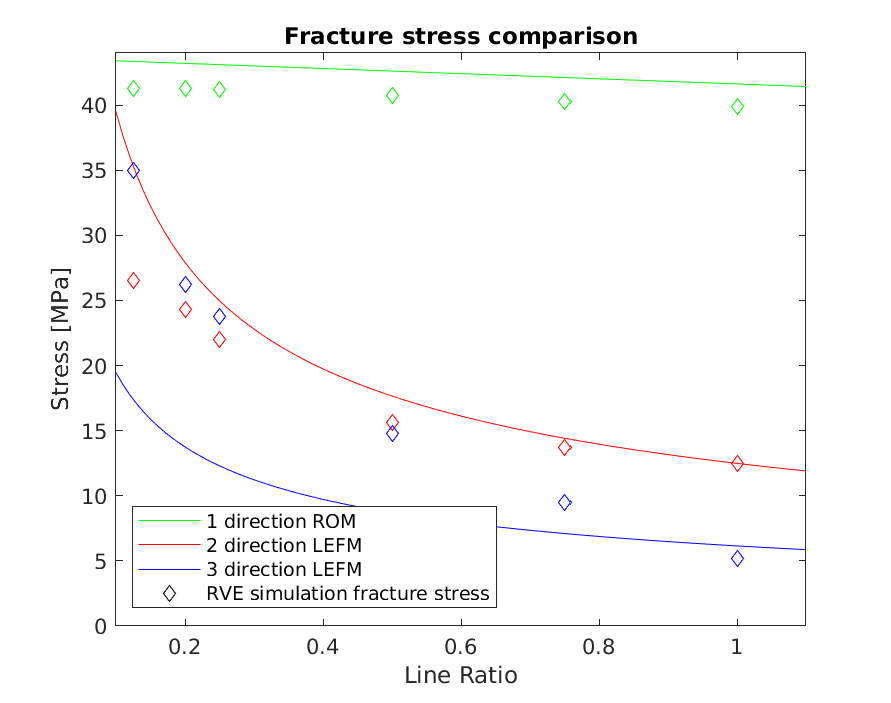
\includegraphics[width=0.80\textwidth]{chapter_7_non-elasticmodelling/figures/yieldstress.png}
    \caption{Comparison between fracture stress of the Stress Intensity approach and the RVE simulations for different aspect ratios}
    \label{fig:fracturestress}
\end{figure}
\subsection{Cracktip plasticity}

In figure \ref{fig:cracktip} the radius for cracktip plasticity is plotted and compared with the distance to the end of the RVE. This would in theory mean that the crack tip plasticity at the point of fracture will always we larger than the distance from the cavity to the end of the RVE, creating a fully brittle failure.  
\begin{figure}[H]
    \centering
    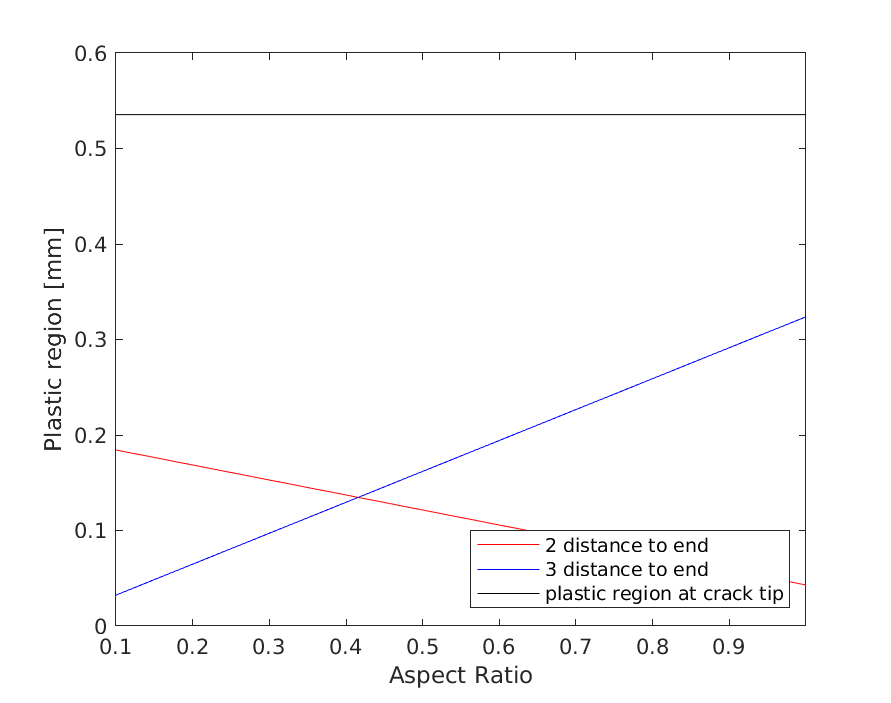
\includegraphics[width=0.80\textwidth]{chapter_7_non-elasticmodelling/figures/cracktip.png}
    \caption{Crack tip plasticity radius for different aspect ratios compared with the distance to the end of the RVE}
    \label{fig:cracktip}
\end{figure}


\section{Discussion}
%mesh convergence
The mesh convergence study shows that the mesh is not fully converged, this means that it might be possible that the results will be altered even more. However, due to the computationally expensive procedure, this is not possible. Additionally, the current results are very close to the empirical obtained stress strain curves, therefore it is probable that this is a mesh close to the representation of the reality. 

%RVE convergence
The RVE convergence procedure was done with a 0.01 coarse mesh. This implies that there would be a possibility that the response for multiple RVE's could be altered for finer meshes. However, due to the limitations in computational power, this study should settle with the assumption that multiple RVE's would not lead to an alteration in results.  

% Comparison SS curves
The comparison between the empirically obtained response using the ASTM D 3039 standard and the RVE simulations for 0.4 mm line width and 0.2 mm layer height who significant overlap in the behaviour of the FFF products. As is discussed in Methods and Procedures, the non-linear behaviour is rather difficult to predict for thermoplastics, however the implemented yield and failure criterion does seem to achieve a reasonable prediction in the 1 direction. The input curve could be optimized to achieve a more overlapping response. As is mentioned in chapter 5 the input curve was obtained from a relatively old filament, which is suspected to have degraded due to UV light and water absorption, resulting in a more brittle response in comparison with the fresh filament that was used for the ASTM D 3039 test samples.
The 2 and 3 direction show significant overlap in its behaviour. The 2 direction almost perfectly predicts the UTS, the difference between the simulated RVE and the empirical test can be accounted to a difference in mesostructure, a sub optimal healing or measurements defects (in chapter 4 it was discussed that the dimensional accuracy of FFF parts are limited, and accurate calculations for the surface might be troublesome). The difference in elasticity might be produced by this phenomenon. To more accurately determine the mechanical properties through experimental test, more data needs to be generated with a optimized testing method. 
Direction 3 predicts the the elasticity relatively good, but has a lower UTS. This is theoretically attributed to the decrease in healing, as is concluded in chapter 4. Additionally, in the work of van Veen \cite{Veen2019EnhancingTemperature}, PETG experimental tests with envelope temperatures close to $T_g$ and room temperature were conducted with ZX[0] samples. These stress strain curves showed the same brittle behaviour and showed a UTS of roughly 26\% of bulk UTS for $T_g-55$ (room temperature) and 36\% for $T_g-15$, which means an increase of 10\% in relative bulk UTS for an almost fully healed part. For the experimental data generated for ABS, the UTS went from 23\% of the UTS for a tensile test at room temperature, to a  34\% relative UTS for simulated fully healed material. This may very well explain the difference between the sub-optimally healed experimental test, and the fully healed simulated RVE (which assumes bulk properties). However, this theory should still be strengthened by additional empirical tests for different temperatures and additional test for the aspect ratios in the 3 direction, both empirically tested and simulated. 
In chapter 5 it was discussed what testing method would generate a most realistic response. The results from the RVE simulations clearly indicates that the ASTM D 3039 standard has a far better correlation, the reasons behind this are discussed in chapter 5.

%aspect ratios
As can be seen in figure \ref{fig:AR1}, the response in the 1 direction does not change significantly for different aspect ratios, this is due to the fact that the surface fraction slightly decreases with an increasing surface fraction, this can be seen figure \ref{fig:Elasticproperties} and is discusses in chapter 4. The response in the 2 and 3 directions significantly alters, due to the difference in surface fraction in the respective directions. As is expected from the theory, and discussed in chapter 6 enough, the elastic moduli in the 2 direction does not change drastically. However, due according to fracture mechanics, the critical stress scales exponentially instead of linearly with elasticity, therefore the stress at fractures significantly decreases with a larger aspect ratio.  In the 3 direction, the surface fraction does change by a large factor (from 0.9 to 0.21 for respectively an aspect ratio of 0.125 and 1), therefore both elastic modulus and fracture stress will drastically change. The smallest aspect ratio (0.125) even shows a ductile response, meaning the porosity might be small enough to decrease the stress concentrations at the tips. Also, a finer mesh might result in a different response as was discussed before. 
According to the simulated results, a smaller aspect ratio will results in better and more isotropic properties in all directions, which is in line with the results generated in the literature. The issue is that the printing time will scale  inversely proportionally with an increase in  aspect ratio, therefore at trade-off should be applied, for engineering applications, an aspect ratio of 0.25 often seems decent. 

%fracture stress 
The prediction of the UTS in the one direction is in reality trivial, one can simply use the Voigt equation \ref{eqn:Voigt} when the mesostructure is known to obtain a decent prediction.  The 2 and 3 directions show significant overlap with the fracture theory. These results also shows overlap with experiments from \cite{Li2017TheProperties} shown in figure \ref{fig:Layerheigth}, however these experiments were conducted with different process parameters and can therefore not be directly compared. The slope of the curve in figure \ref{fig:fracturestress} (which is governed by the exponent operator), and the magnification (which is governed by an empirically determined factor) could be altered to produce a fitted equation, but before implementing this, a more extensive mesh convergence study needs to be performed. This is however not part of this thesis, it is sufficient to conclude a significant overlap between linear elastic fracture mechanics to predict the fracture behaviour of FFF parts since the porosity can behave like microcracks. 

%contour plots
The contour plots show the stress concentrations at the crack tips for the 2 and 3 directions. These stress concentrations have the same form as is predicted in plane strain fracture mechanics (figure\ref{fig:stresscrack}), which indicated the relevance for the application fracture mechanics theory. In the contour plots for the 1 direction, shear bands are observed for the strain contour plots. This is due to the yield criterion (equation \ref{eqn:Tschoegl}), which dictates a yield loci that will deform plastically in shear. Due to the applied positive Poisson ratio a certain shear stress will develop once the material is loaded in tensile, therefore the material will develop larger strains due to these shear bands, and will finally will fail in this region due to the strain based failure criterion \ref{eqn:JC}. This is in line with polymer science as is discussed in chapter 2, where polymers loaded in tensile will form shear bands and will finally fail due to the maximum strain of a polymer molecule. The contour plots additionally show the formation of the crack, which in most cases is perpendicular to the loading face, starting at the cavity tip. 

%crack tip plasticity
Finally, the prediction of the crack tip plasticity indicates that a fully healed FFF product will exhibit plasticity at the crack surface. This is in line with the empirical observations of tested samples produced at high envelope temperature (showing whitened regions, indicating shear band or crazing), while samples produced at room temperature did not show any whitening, indicating sub optimal healing. This might serve as a visual inspection method to confirm full healing was achieved. 
%



\section{Conclusion}
After the mesh convergence study and optimization of the FEM analysis, a result was generated for a 0.5 aspect ratio that shows significant overlap with the experimental tests from the ASTM D 3039 standard. The 1 and 2 direction show a variation of less than 5\% percent in the determination of the UTS, the elongation is more difficult to determine since polymers have a complex strain (rate) dependency. Nonetheless, the strain at break is also predicted inside an acceptable margin (since the standard deviation of empirical results in strain is also significant). The 3 direction from the simulated shows a difference in UTS compared to the empirical results due to the worse bonding between layers, this is exactly in line with the healing theory which has been explained in literature, however, this effect seems to be significantly less pronounced than first was assumed. According to the obtained results in this thesis, for ABS specimen printed at room temperature, the porosity has a major influence compared to sub-optimal healing.  The healing effect in the 2 direction is minimal (less than 5\% decrease of the orginal UTS), since the toolhead quickly reaches the same spot before cooling. This will obviously differ for different geometries and speeds. In the 3 direction, the healing effect would be most significant, and is responsible for a decrease in UTS of roughly 10\% of decrease in mechanical properties. This therefore means that, with these process parameters, that porosity is by far the dominant influencer of mechanical properties, with more than 90\% in every direction. This decrease in mechanical properties is most present in the 2 and 3 direction, where the UTS decreases with more than 65\%, additionally the E modulus is decreased with as much as 70\%. 
The Linear Elastic Fracture mechanics show significant resemblance with the results derived from the RVE simulations. Further research into the porosity for different aspect ratios might give more tools to predict the fracture behaviour with analytical approaches. 
As is expected from literature, the decrease in aspect ratio significantly increases the mechanical properties of FFF products, due to the reduced porosity. However, this comes as at a cost of increased printing time.
To also validate the RVE model for the aspect ratios used, empirical tests should be performed with the same aspect ratios. If these also seem to provide corresponding results, different combinations of RVE's could be simulated to replicate layer orientations and hopefully determine the best layer build up. 
Finally, different materials could be used in this model. The same procedure to determine the hardening curve should be applied as is explained in chapter 5. Carbon fibres could help increase the fracture toughness, fibres could obstruct cracks to propagate trough the sample.  
%wait to write after discussion with Miguel

%Interesting to notice is that RVE part should first plastically (ductile failure) deform before rupture (graph), but this doesn't happen since bad inrter layer bonding. 


